\appendix
\section*{Приложение Б: Визуальный результат реализованных методов}
\addcontentsline{toc}{section}{Приложение Б: Визуальный результат реализованных методов}
\label{sec:Apendix2} \index{Apendix2}

\subsection*{Марширование лучей без аккреционного диска}
\addcontentsline{toc}{subsection}{Марширование лучей без аккреционного диска}

\begin{figure}[H]
    \centering
    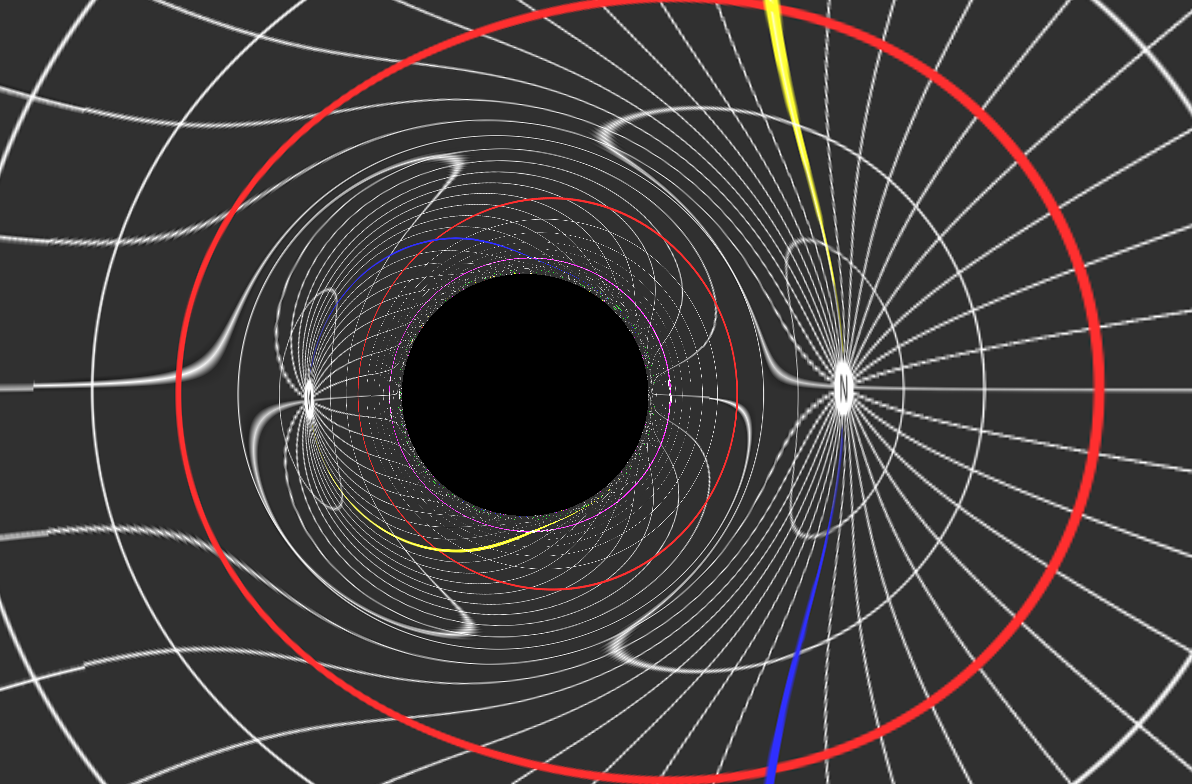
\includegraphics[width=1.0\linewidth]{appendix/UV1}
\end{figure}

\begin{figure}[H]
    \centering
    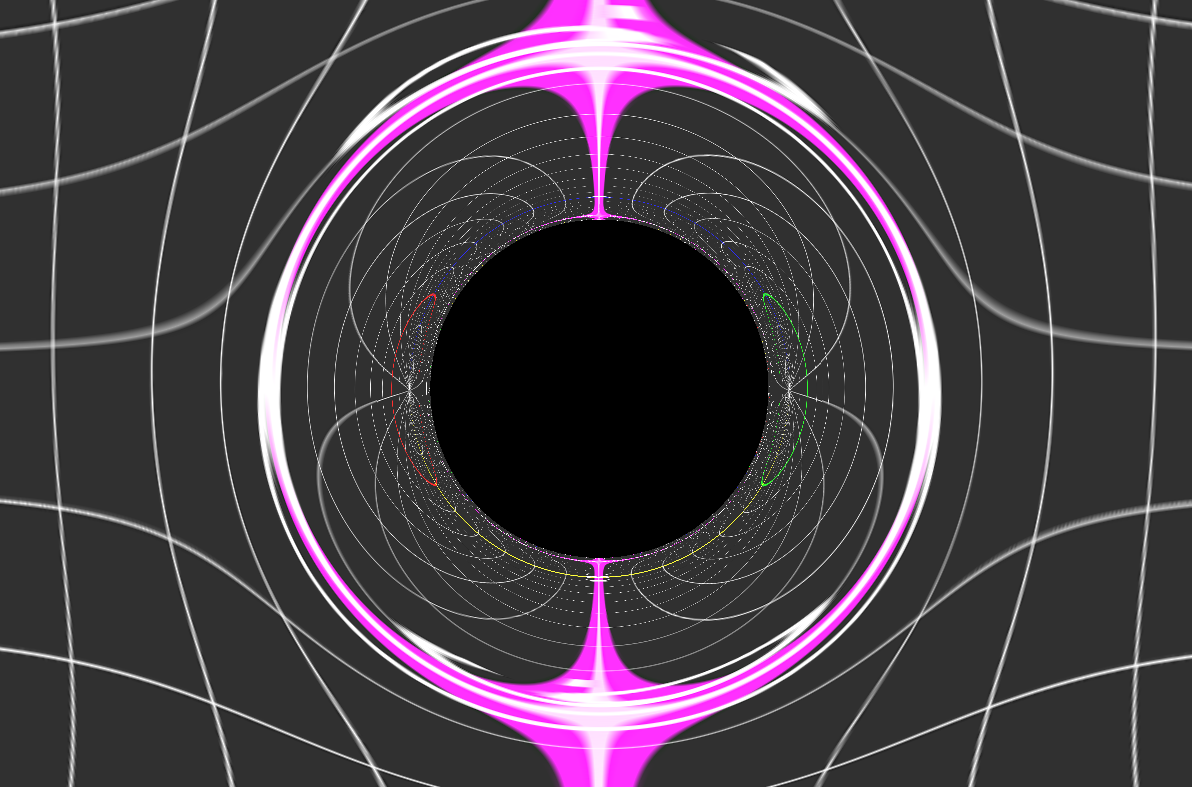
\includegraphics[width=1.0\linewidth]{appendix/UV2}
\end{figure}

\begin{figure}[H]
    \centering
    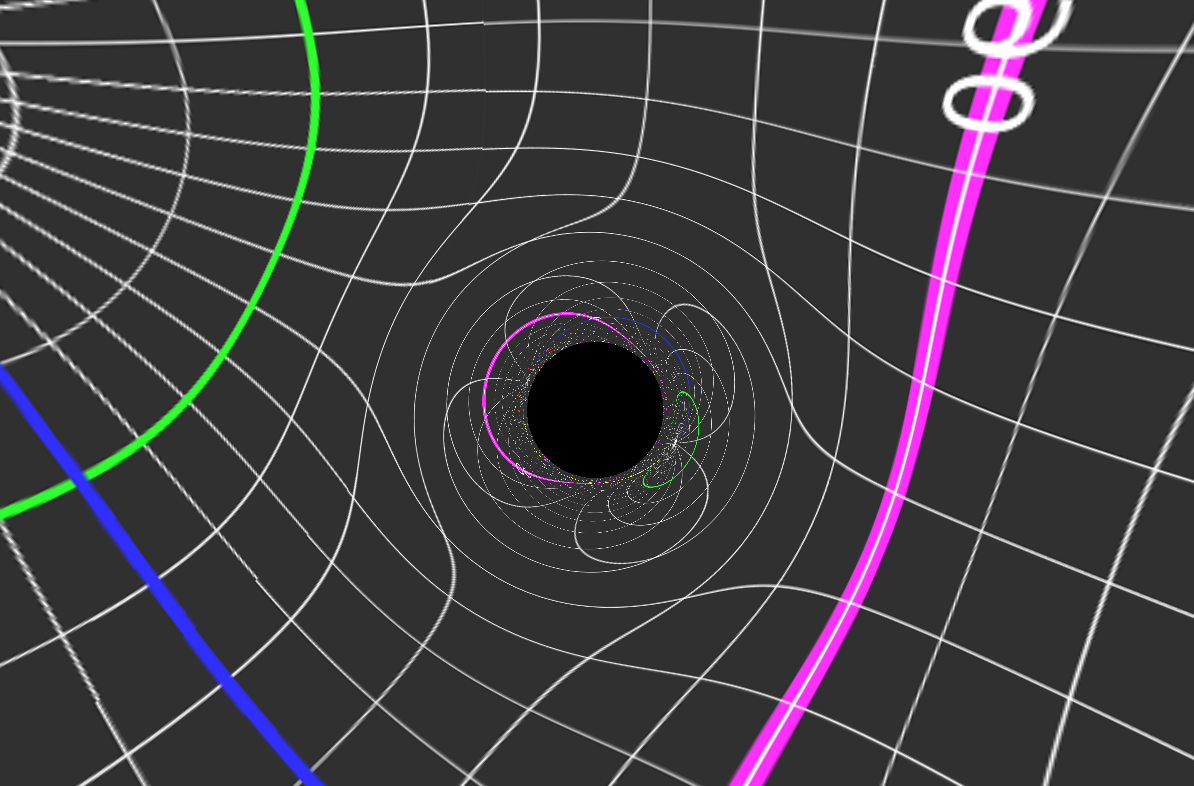
\includegraphics[width=1.0\linewidth]{appendix/UV3}
\end{figure}

\begin{figure}[H]
    \centering
    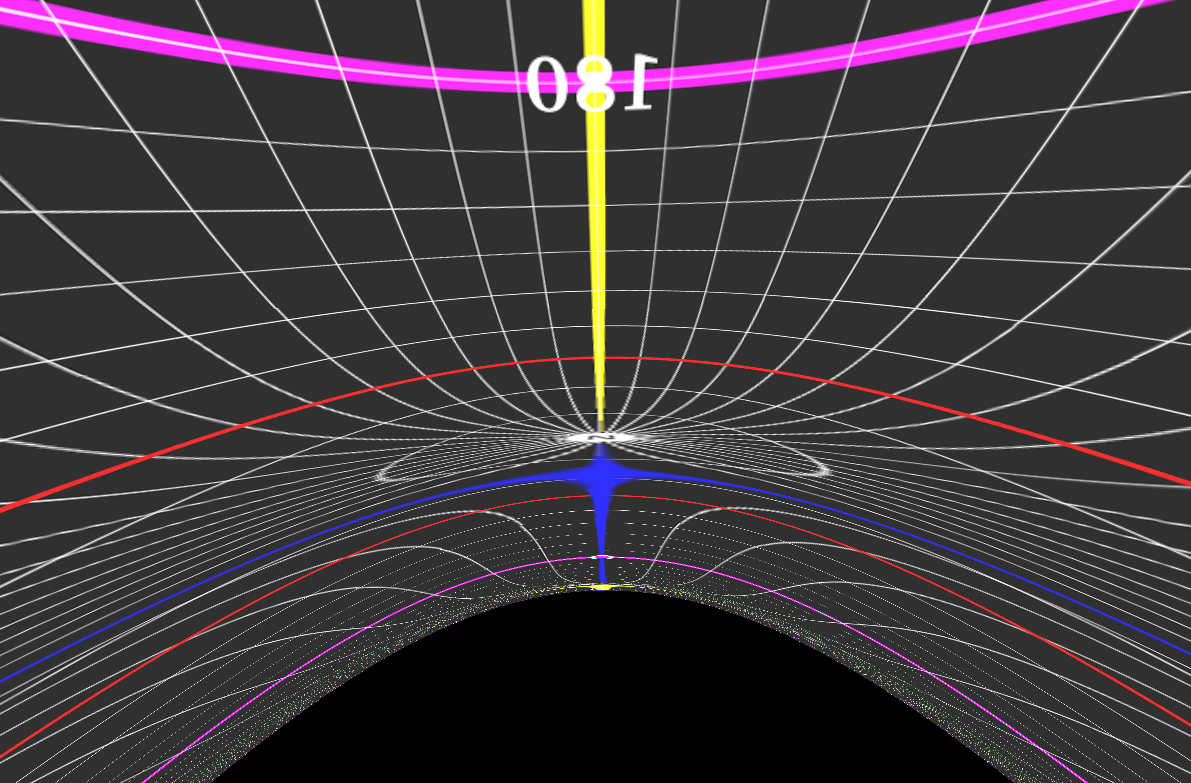
\includegraphics[width=1.0\linewidth]{appendix/UV4}
\end{figure}

\subsection*{Марширование лучей}
\addcontentsline{toc}{subsection}{Марширование лучей}

\begin{figure}[H]
    \centering
    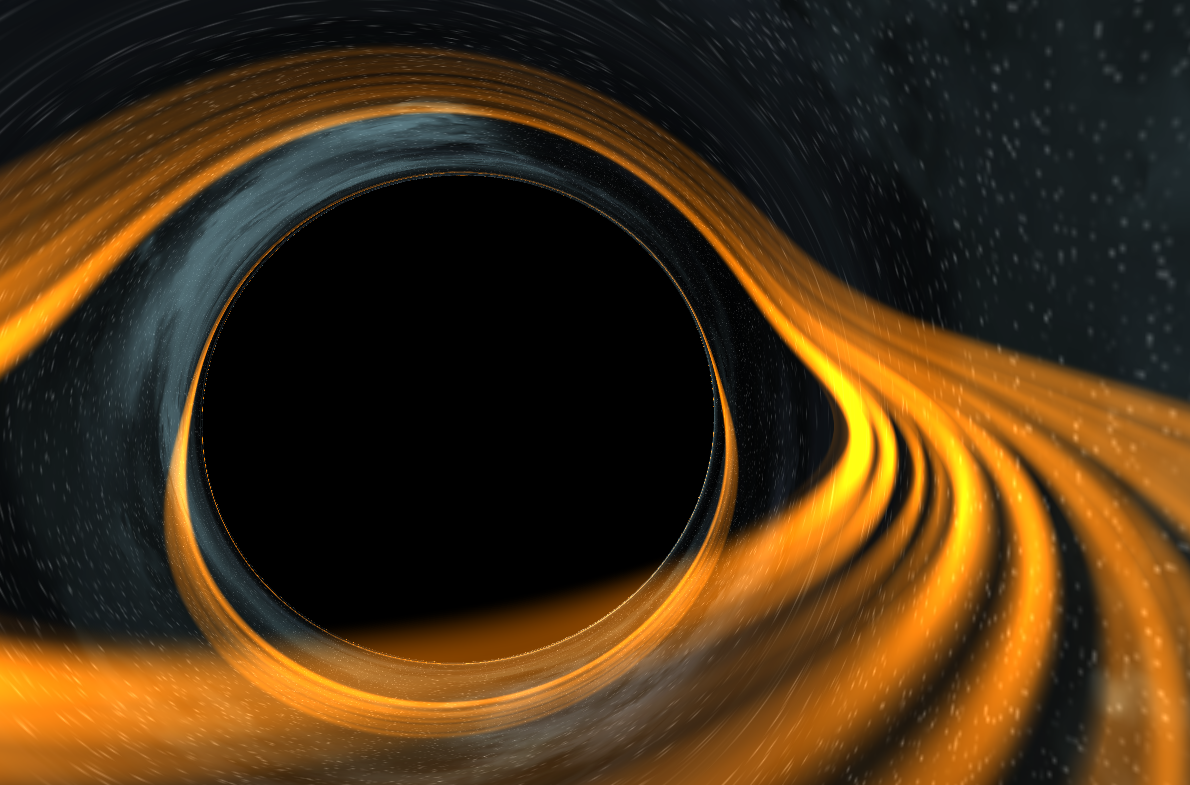
\includegraphics[width=1.0\linewidth]{appendix/RM1}
\end{figure}

\begin{figure}[H]
    \centering
    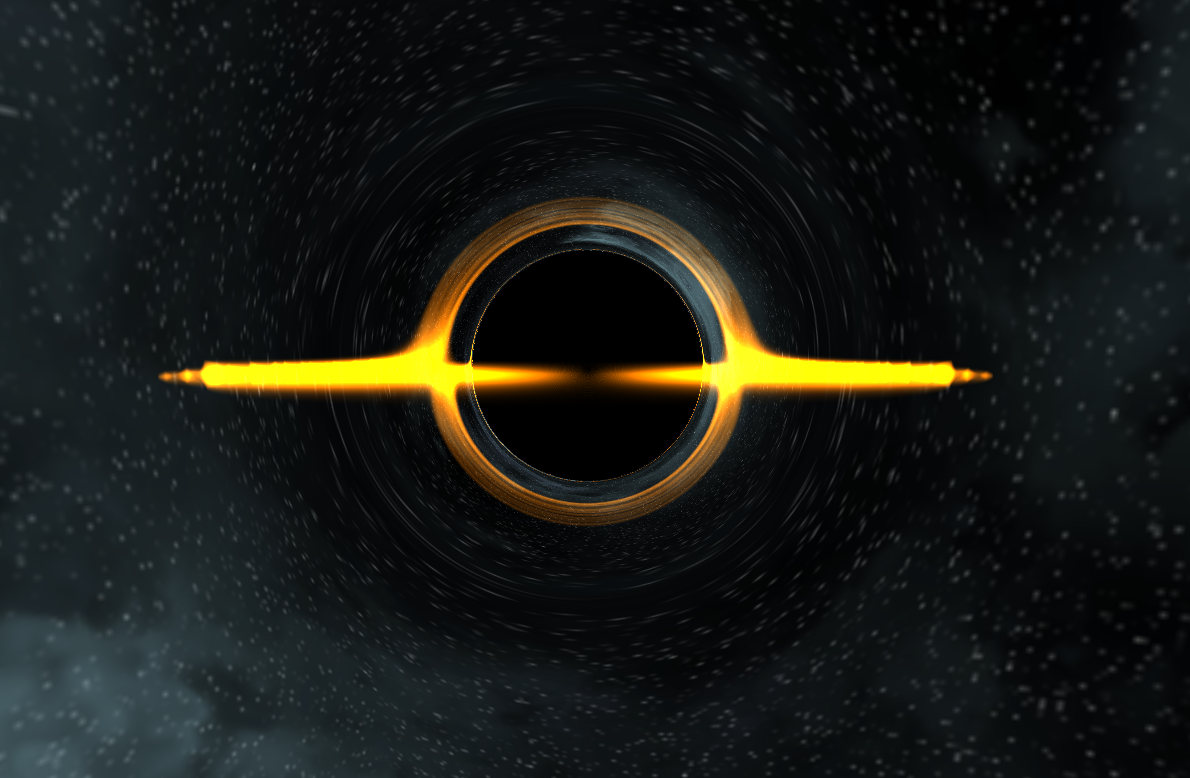
\includegraphics[width=1.0\linewidth]{appendix/RM2}
\end{figure}

\begin{figure}[H]
    \centering
    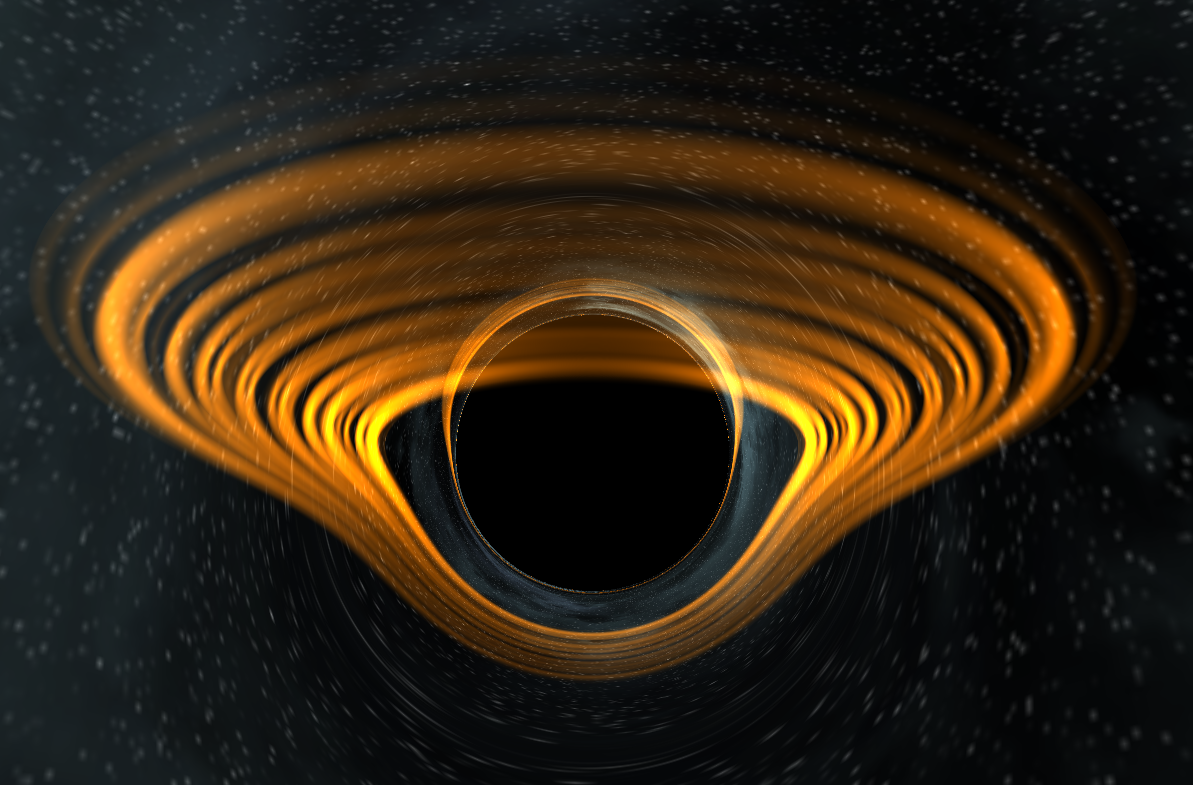
\includegraphics[width=1.0\linewidth]{appendix/RM3}
\end{figure}

\subsection*{Предрасчитанные данные}
\addcontentsline{toc}{subsection}{Предрасчитанные данные}

\begin{figure}[H]
    \centering
    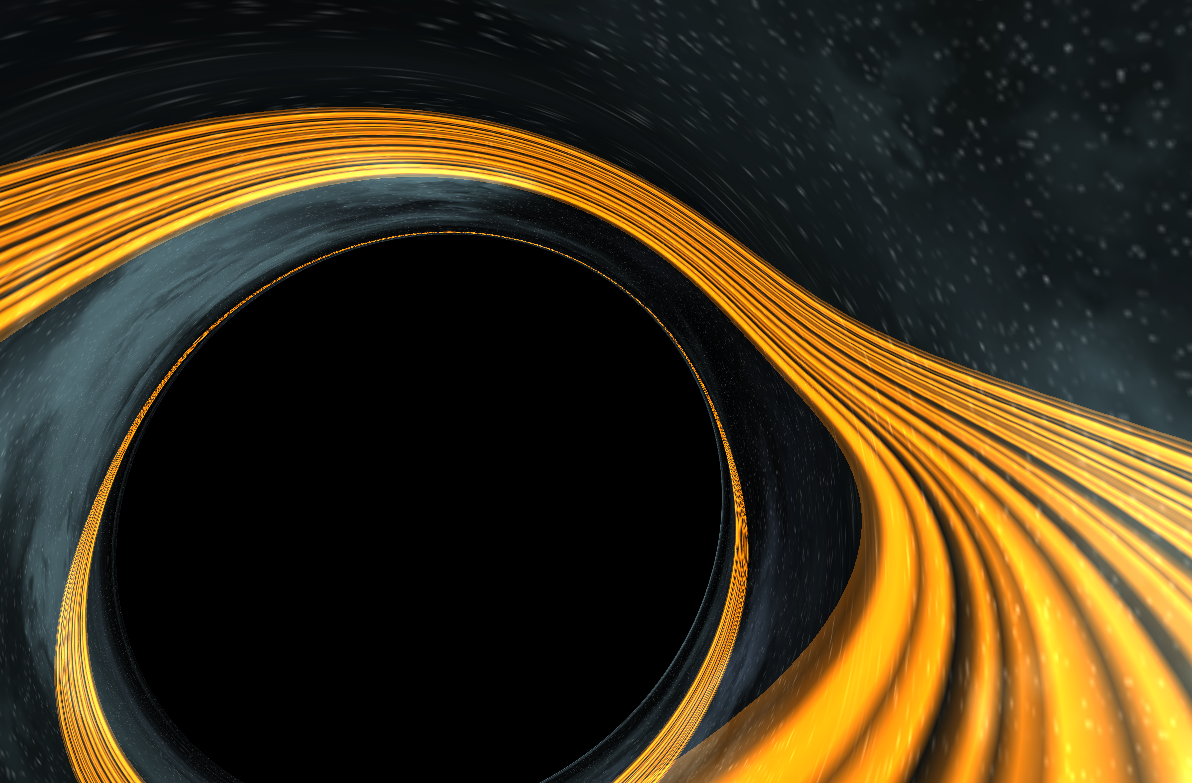
\includegraphics[width=1.0\linewidth]{appendix/PD1}
\end{figure}

\begin{figure}[H]
    \centering
    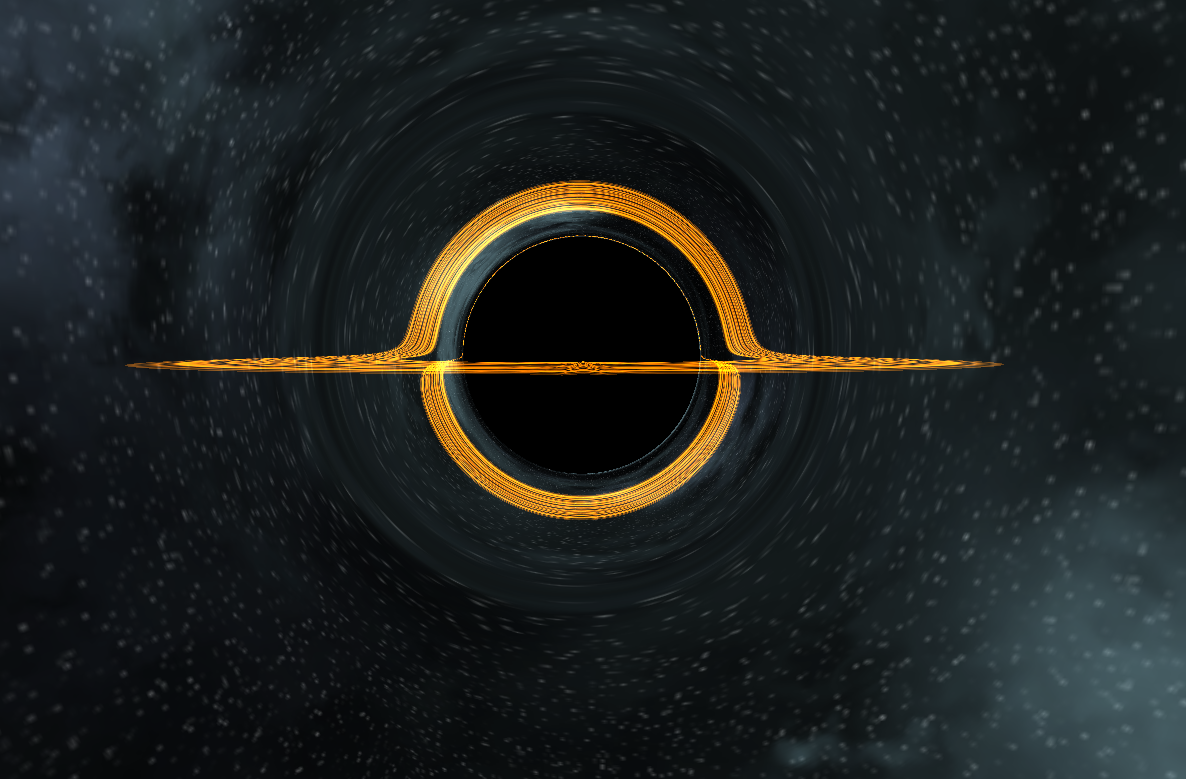
\includegraphics[width=1.0\linewidth]{appendix/PD2}
\end{figure}

\begin{figure}[H]
    \centering
    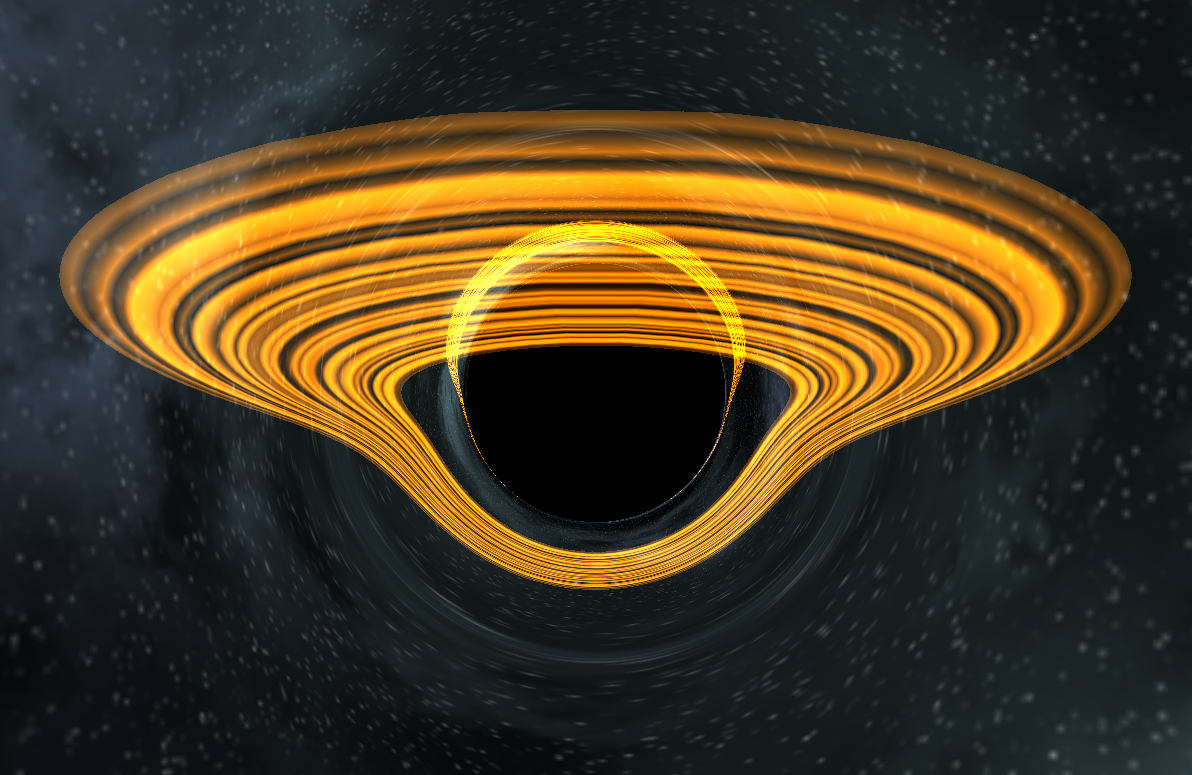
\includegraphics[width=1.0\linewidth]{appendix/PD3}
\end{figure}

\subsection*{Марширование лучей и трассировка лучей}
\addcontentsline{toc}{subsection}{Марширование лучей и трассировка лучей}

\begin{figure}[H]
    \centering
    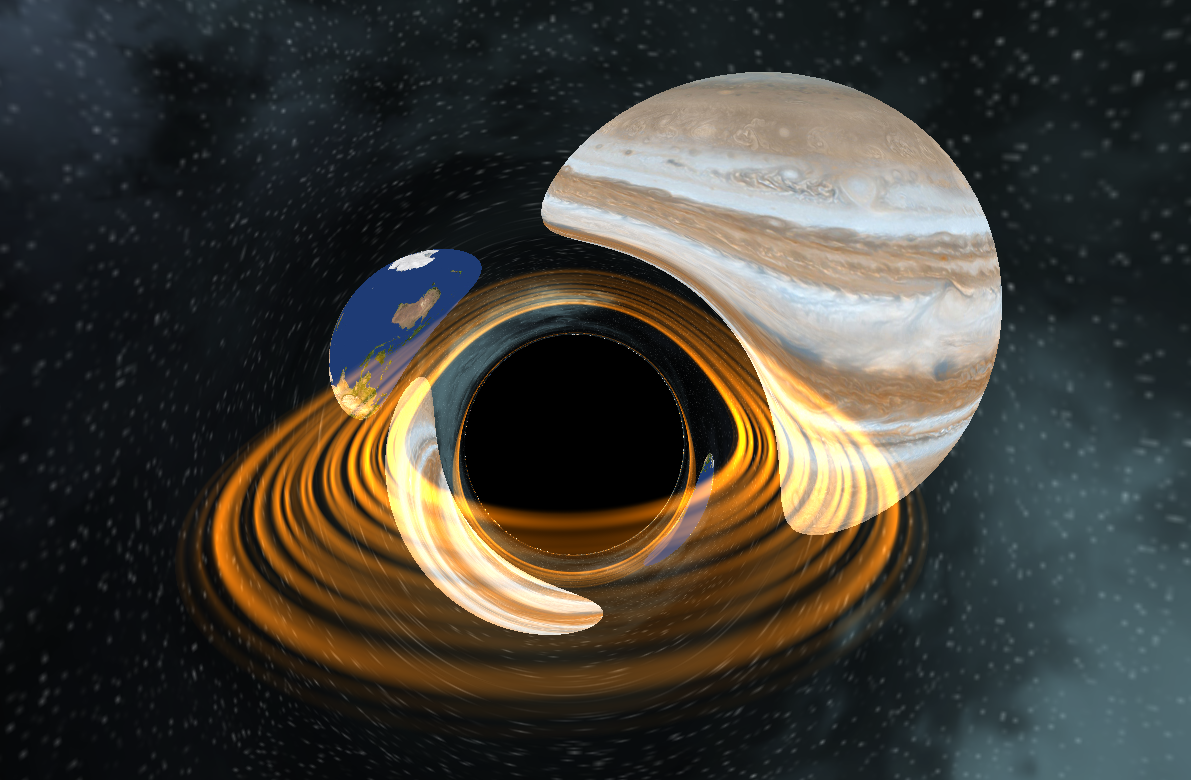
\includegraphics[width=1.0\linewidth]{appendix/RMT1}
\end{figure}

\begin{figure}[H]
    \centering
    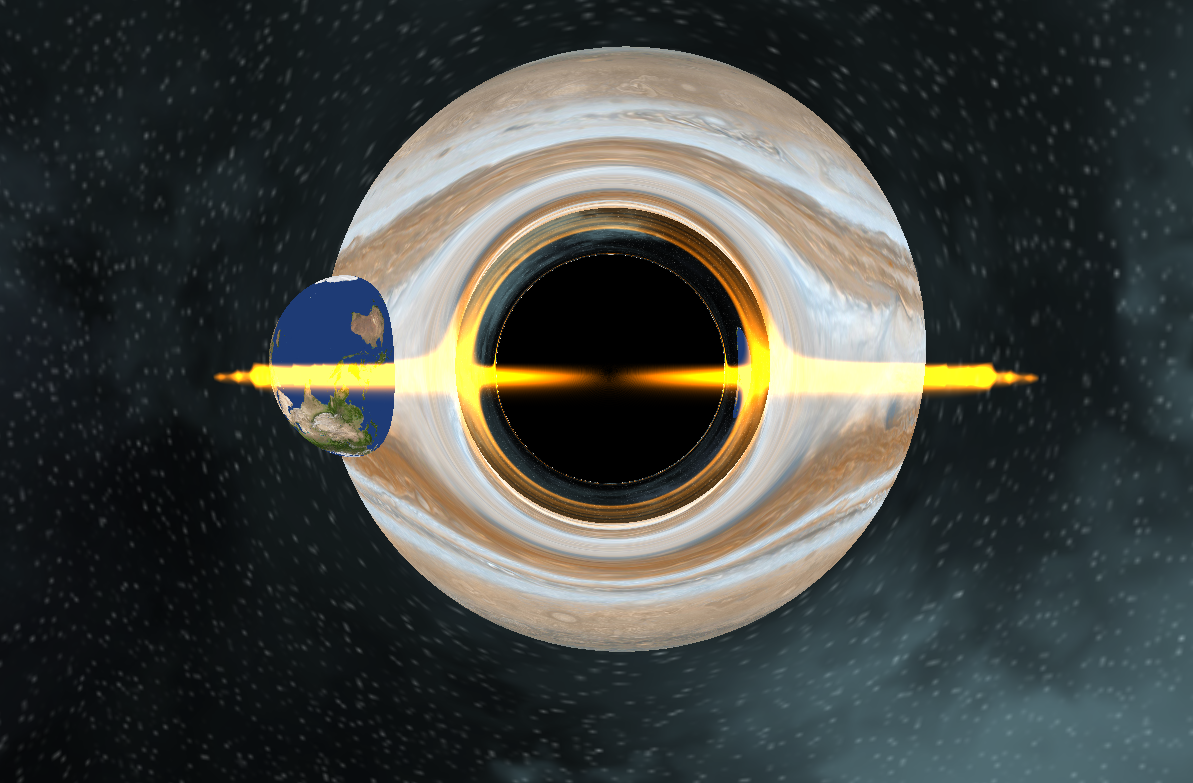
\includegraphics[width=1.0\linewidth]{appendix/RMT2}
\end{figure}

\begin{figure}[H]
    \centering
    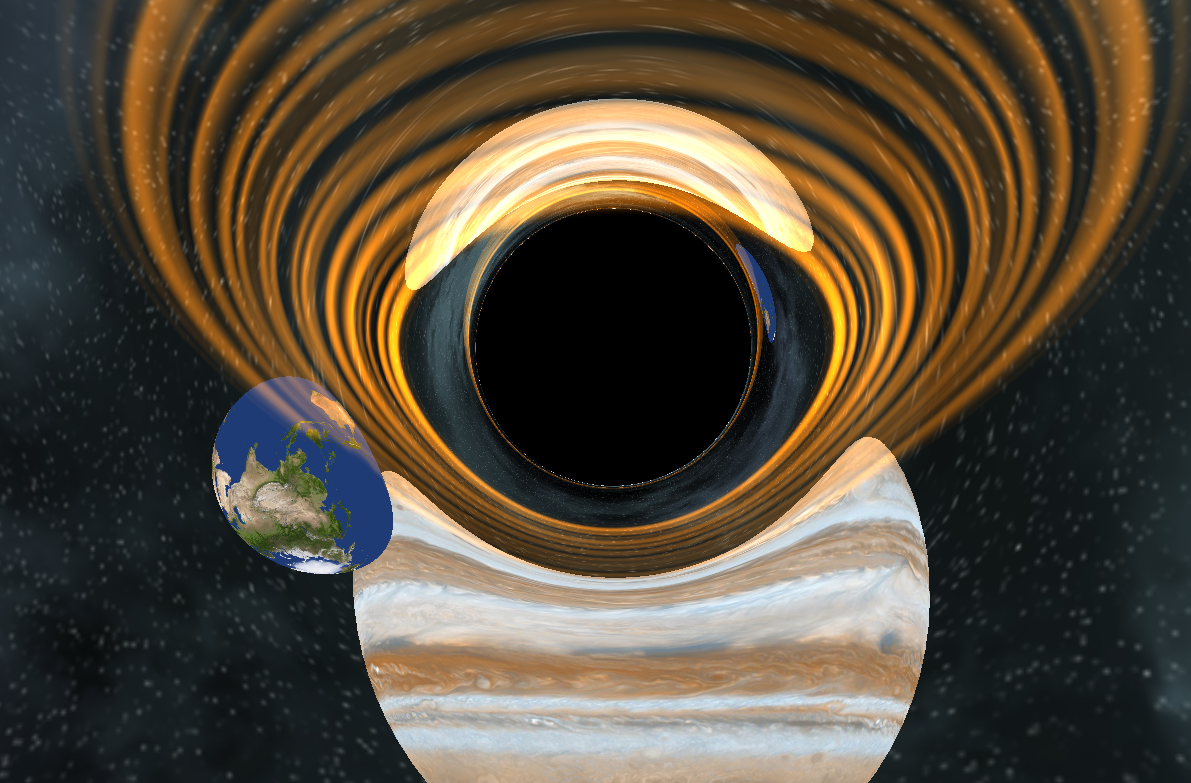
\includegraphics[width=1.0\linewidth]{appendix/RMT3}
\end{figure}

\subsection*{Двойная черная дыра}
\addcontentsline{toc}{subsection}{Двойная черная дыра}

\begin{figure}[H]
    \centering
    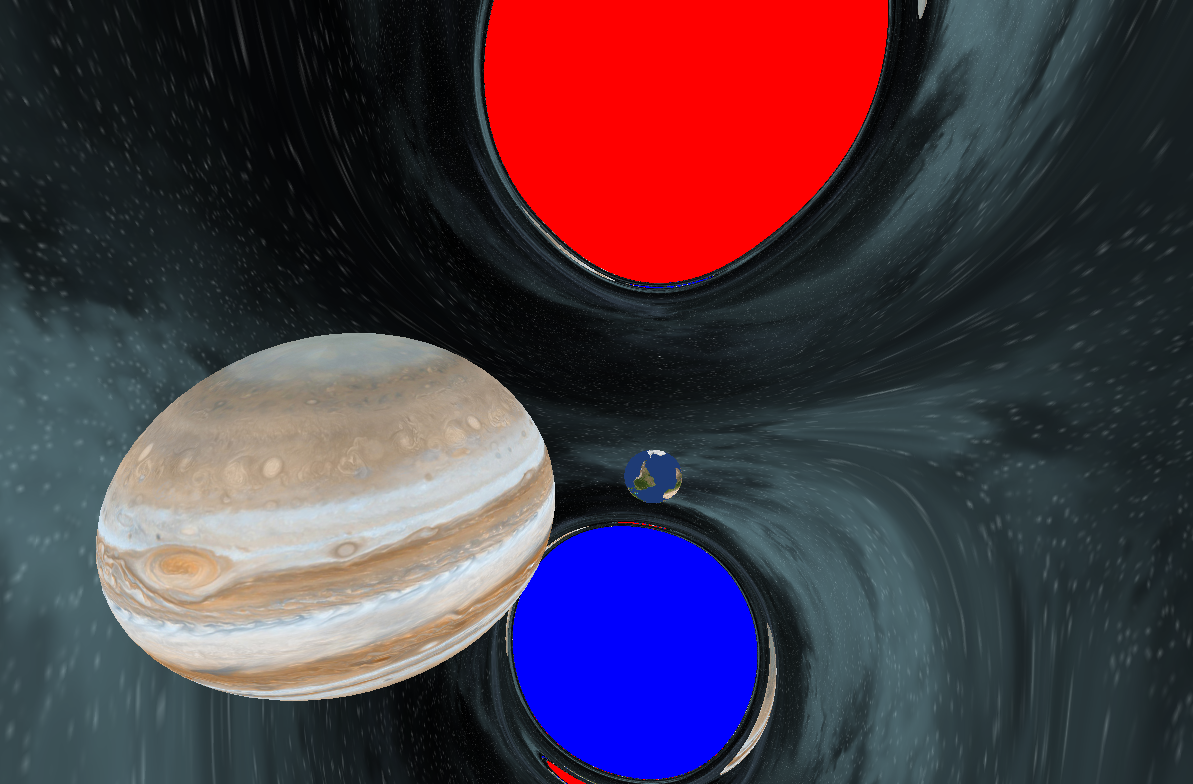
\includegraphics[width=1.0\linewidth]{appendix/2BH1}
\end{figure}

\begin{figure}[H]
    \centering
    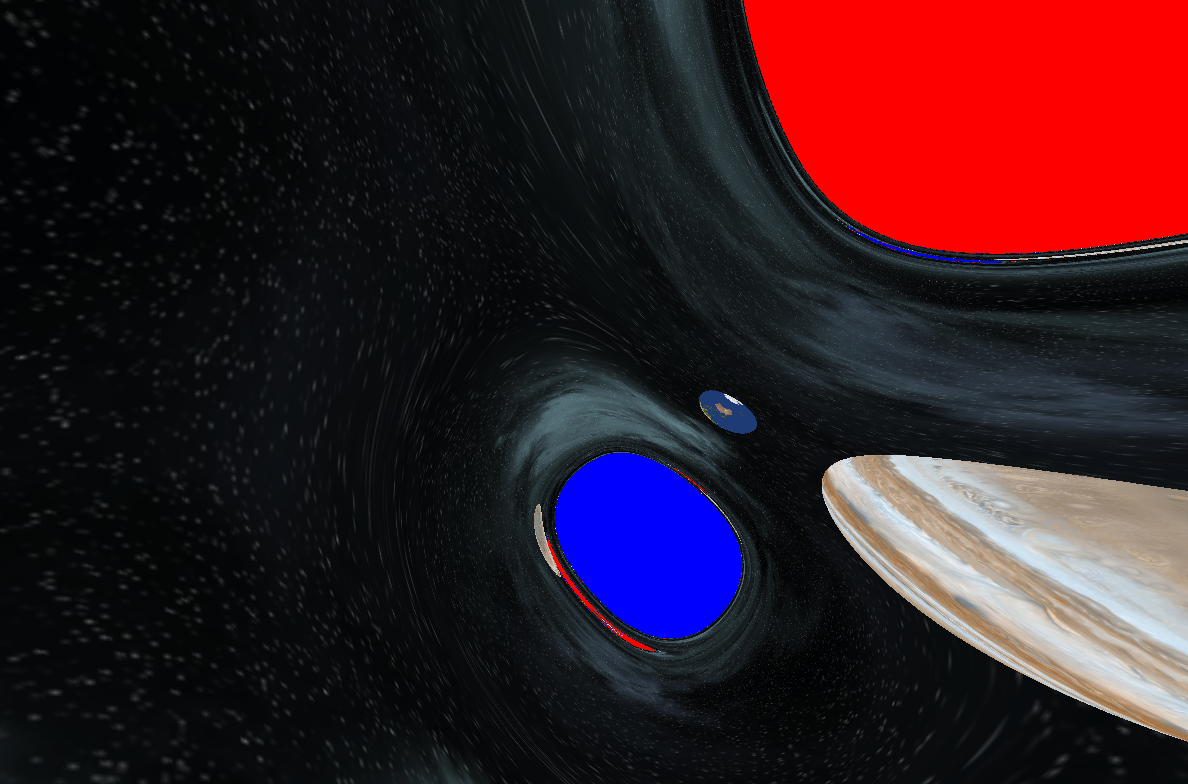
\includegraphics[width=1.0\linewidth]{appendix/2BH2}
\end{figure}

\newpage